\section{Resolución Problema 2} 
En el siguiente informe se emplea la metodología de las 6 D´s, el cual tiene como objetivo presentar el desarrollo y los resultados obtenidos de la elaboración de un programa en Java que permite resolver ecuaciones cuadráticas utilizando la fórmula general, dando lugar a tres posibles resultados.
\subsection{\textbf{Descripción del problema:}}
Dada una ecuación cuadrática regresar los valores de las raíces en caso de que estén sobre el conjunto de los números reales, en caso contrario indicar que la solución está en el conjunto de los números complejos. El principal objetivo será encontrar el valor de “x” para lograr que la ecuación sea verdadera.
\subsection{\textbf{Definición de solución:}}
La forma general de la ecuación de segundo grado es la siguiente:

\begin{equation}
    ax^{2}+bx+c=0  
    \label{eqn:ecuacioncuadratica}
\end{equation}
A continuación se muestra la fórmula general, con la cual se realiza la sustitución de los valores correspondientes a “a”, “b” y “c” de acuerdo a la ecuación de segundo grado (1) que se desee resolver y por ende, conocer su resultado.

\begin{equation}
    \frac{-b\pm\sqrt{b^2-4ac}}{2a}
\end{equation}

Es importante saber que el resultado puede variar en ninguna, una o dos soluciones reales.

La representación gráfica es la siguiente:

\begin{figure}[!ht]
\centering
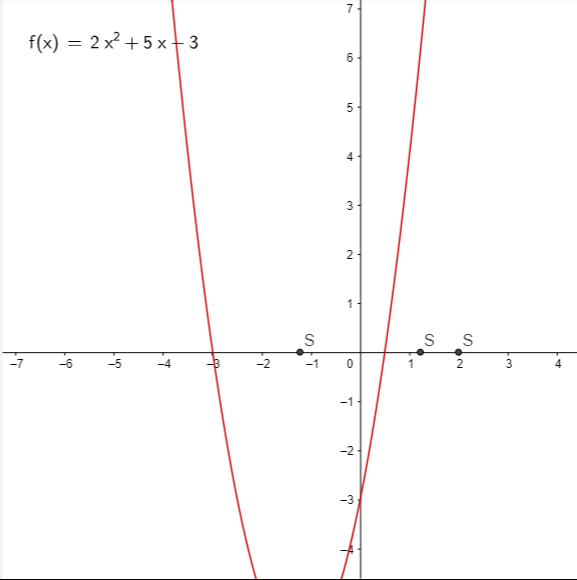
\includegraphics[width=6cm]{LaTeX/latex-imagenes/ejemploGrafica.png}
\caption{Gráfica de una ecuación cuadrática con dos soluciones.}
\label{fig:grafica}
\end{figure}

\newline
\subsection{\textbf{Diseño de la solución:}}
Para lleva a cabo la elaboración del código de java, se requiere diseñar el proceso para asegurar que el progreso sea correcto.

%diagrama
\begin{figure}[H]
\centering
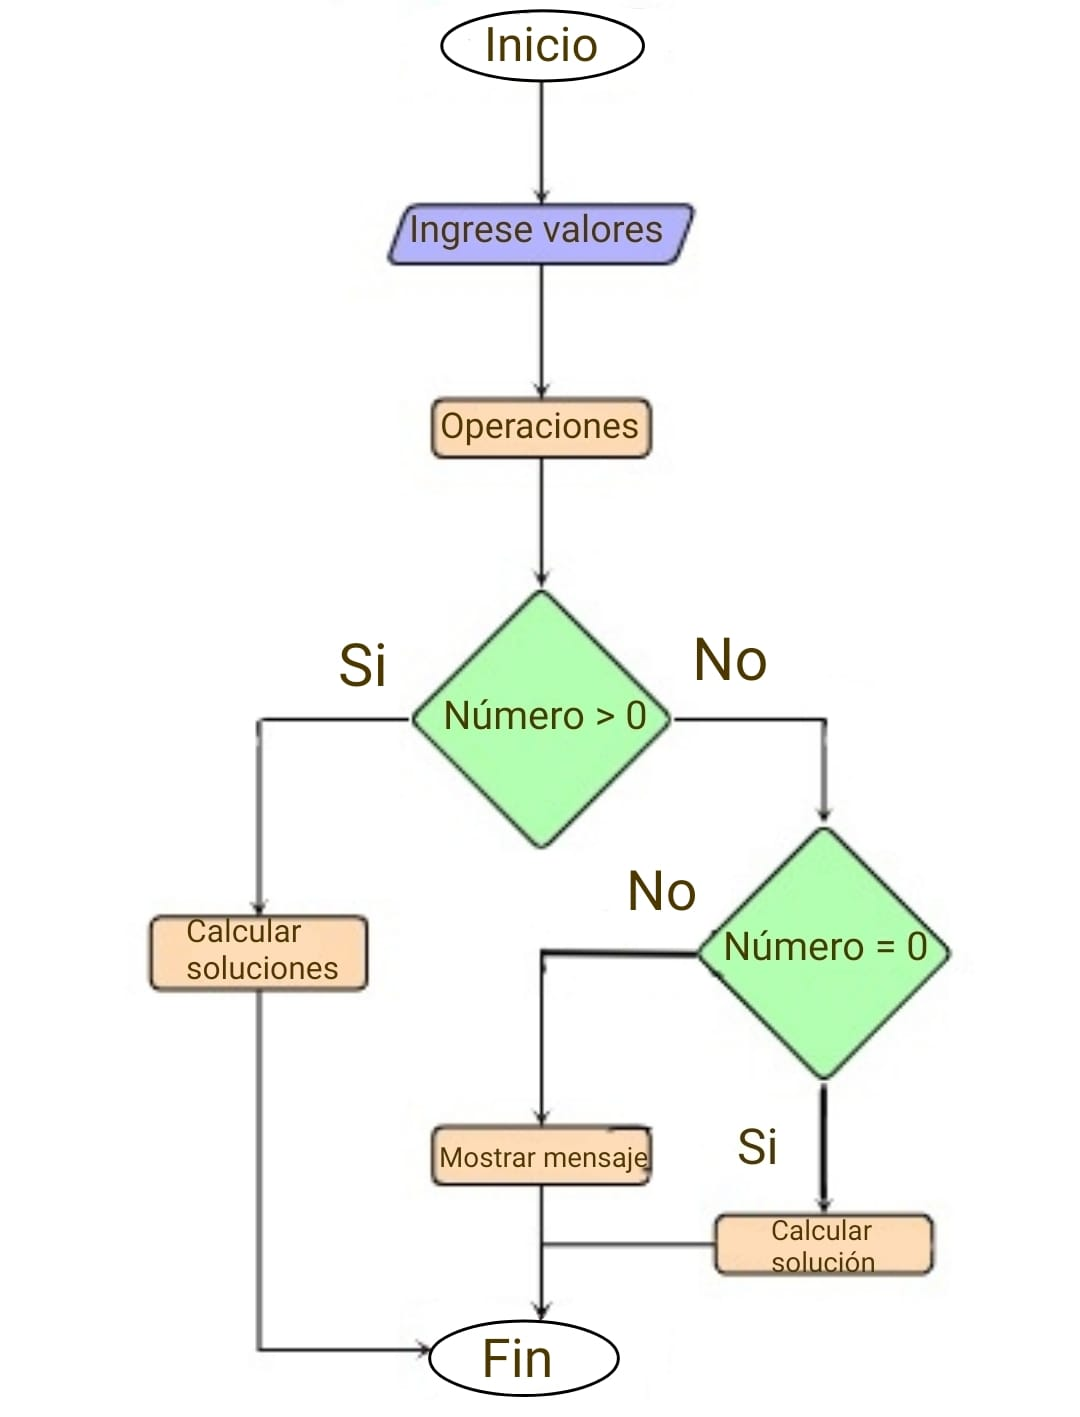
\includegraphics[width=6cm]{LaTeX/latex-imagenes/diagramaflujo.jpg}
\caption{Diagrama de flujo que muestra el proceso para resolver la fórmula general.}
\label{fig:diagrama_flujo}
\end{figure}

\newline

Prosiguiendo con el diseño, ahora se va a mostrar el código como resultado de la elaboración del diagrama donde:

\begin{itemize}
  \item El usuario debe ingresar tres valores, es decir, los coeficientes pertenecientes a la forma estándar de la ecuación cuadrática.
  \item El programa realiza las operaciones correspondientes a la fórmula general.
  \item Al final el o los resultado serán mostrados.
\end{itemize}
\subsection{\textbf{Desarrollo de la solución:}}
\subsection{Programa en Java}
En seguida, se muestra el código del programa.
Se utiliza la clase Scanner y la clase Random que se encuentran en el paquete de java.util, y además se agrega el tipo de dato.

\begin{lstlisting}[style=javaStyle]
public static void main(String[] args) {
        Scanner constante = new Scanner(System.in);

        double a, b, c, numero, x1, x2, x;
\end{lstlisting}
**
%codigo
El usuario ingresa los valores solicitados, siendo las variables ``a", ``b'' y ``c". Posteriormente se cierra el escaneo.

\begin{lstlisting}[style=javaStyle]
//Solicita el valor de los coeficientes para realizar la ecuación
        System.out.print("Ingrese el valor de a: ");
        a = constante.nextDouble();
        
        System.out.print("Ingrese el valor de b: ");
        b = constante.nextDouble();
        
        System.out.print("Ingrese el valor de c: ");
        c = constante.nextDouble();
        //Cierra el escaneo
        constante.close();

\end{lstlisting}

Continúa cerrando  y a realizar las primeras operaciones de la fórmula general, que serán determinantes para la siguiente condición de la estructura de control if.

\begin{lstlisting}[style=javaStyle]
        //Cierra el escaneo
        constante.close();
        
        numero = b * b - 4 * a * c;
\end{lstlisting}
Prosiguiendo con la operación de la fórmula general, ahora se debe determinar cuál será la respuesta dependiendo del resultado de la operación anterior, entonces la estructura de control if va a permitir tomar decisiones en función de la condición y así llegar a un resultado.

\begin{lstlisting}[style=javaStyle]
   //Se va a determinar cuál de las tres posibles soluciones es 
       // la indicada dependiendo de los valores ingresados
        if (numero > 0) {
            x1 = (-b + Math.sqrt(numero)) / (2 * a);
            x2 = (-b - Math.sqrt(numero)) / (2 * a);
            System.out.println("Tiene dos soluciones, las cuales son x1 = " + x1 + " y x2 = " + x2);
        } else if (numero == 0) {
            x = -b / (2 * a);
            System.out.println("Solo tiene una solución, la cual es x = " + x);
        } else {
            System.out.println("La ecuación no tiene soluciones reales.");
        }
\end{lstlisting}
 Después de que la condición evaluada sea verdadera, procede a imprimir en la consola el resultado de las operaciones de la fórmula general realizadas junto con el mensaje correspondiente.

\subsection{Código completo}
\begin{lstlisting}[style=javaStyle]
import java.util.Scanner;

public class ecuacionCuadratica {

    public static void main(String[] args) {
        Scanner constante = new Scanner (System.in); 
        
       double a, b, c, numero, x1, x2, x;
        //Solicita el valor de los coeficientes para realizar la ecuación
        System.out.print("Ingrese el valor de a: ");
        a = constante.nextDouble();
        
        System.out.print("Ingrese el valor de b: ");
        b = constante.nextDouble();
        
        System.out.print("Ingrese el valor de c: ");
        c = constante.nextDouble();
        //Cierra el escaneo
        constante.close();
        
        numero = b * b - 4 *a * c;
        //Se va a determinar cuál de las tres posibles soluciones es la indicada dependiendo de los valores ingresados
        if (numero > 0){
            x1 = (-b + Math.sqrt(numero)) / (2* a);
            x2 = (-b - Math.sqrt(numero)) / (2* a);
            System.out.println("Tiene dos soluciones, las cuales son x1 = " + x1 + " y x2 = " + x2);
            
        } else if (numero == 0){
            x = -b / (2*a);
            System.out.println("Solo tiene una solución, la cual es es x = " + x);
        }else {
            System.out.println("La ecuación no tiene soluciones reales.");
        }
    }
}



\end{lstlisting}
\subsection{\textbf{Depuración y pruebas:}}
Comprobación del funcionamiento a través de pruebas, ingresando los valores solicitados al usuario y ejecutando en Java, un total de cinco veces.
\begin{figure}[!ht]
\centering
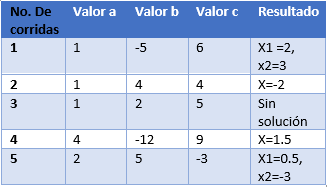
\includegraphics[width=6cm]{LaTeX/latex-imagenes/tablaprueba.png}
\caption{Prueba de escritorio.}
\label{fig:diagrama_flujo}
\end{figure}